\documentclass[12pt]{article}
\setlength{\parindent}{0pt}
\usepackage{setspace}
\usepackage{biblatex}
\usepackage[T1]{fontenc}
\usepackage{titling}
\usepackage{graphicx}
\usepackage{subcaption}

\addbibresource{cite.bib}
 \linespread{1.25}
% Margins
\topmargin=-0.45in
\evensidemargin=0in
\oddsidemargin=0in
\textwidth=6.2in
\textheight=9.0in
% \headsep=0.25in

% \setlength{\droptitle}{-5em}

\title{Group Report \\ Cat People VS Dog People}

\author{Waiting}

\date{\vspace{-8ex}}

\begin{document}
\maketitle

\newpage

\tableofcontents
\newpage

\section{Problem identification}

As we always like to put specific tags to other people to make people into groups to make things easier to understand, 'cat people and dog people' is one of these examples. We get the idea from a research paper which comes from the Facebook\cite{lada}.

After reading the research material, we make an assumption that cat people and dog people have some differences in the respect of movie type preference, book type preference as well as the degree of activity. The objective of our project is to find out what differences are exactly. Besides, we also want to identify whether other aspects have some diversities, such as their location and their sentiment to express on social media.


\section{Data collection}

To find out what are the differences between these two groups in the these aspects, we choose two largest groups of cat and dog respectively. The number of members in cat group is 337,238 and the number in dog group is 156,360, which is enough for our analysis.

After that, we randomly pick 80,000 people from each group with location information to analyze. We also randomly pick 2,000 people from each group and extract the movie and book preference as well as the number of a follower, how many people they follow and how many groups did they visit recently.

To avoid the effect of culture environment, we get 2,000 users from Twitter to compare the distribution of the data to see if culture will affect the result or not. The users we pick has been cleaned already and there is no overlapping between these two tables.

We also crawl data From Twitter API. We search only cat and dog hashtags as keywords instead of using cat and dog directly to avoid some meaningless tweets. The data also be cleaned to avoid overlapping.

% The program we use to crawl all the users with their user ids from each group is 'userIDCrawler.py'. Then, for each individual user, we crawl his/her favorite books and movies. The source code is in the ‘getDetails.py’. What is more, the location of each member, how many fans and how many followings as well as the number of group they visit are extract from the website. The source code is in the 'getFriends.py'. Finally, for each book and movie, we collect its types and tags to build the feature vectors for each movie and book. The source code is in the 'getTags.py'.

\section{Movie Analysis}


\subsection{Data preprocessing}

We define the cat people and dog people as people who join the corresponding group. So, we use SQL to remove the users who join both of the groups. The number of this kind of users is 12,663.

\subsection{Feature engineering}

Firstly, we build the feature vector for each movie and book. The attributes for movie are 37 types of movie and the attributes for book are 3,840 types of tags. The value in the vector are the binary values. Then, we sum up each users' the feature vectors and do the normalization. Because users are chosen randomly, some of them put no movie or book preference information on Douban. For this kind of users, We set their scores of each attribute with evenly number ($\frac{1}{37}$ for movie and $\frac{1}{3840}$) to indicate that they have not particular preference. The feature vectors are put into the data frame of pandas. $M(u)$ is the movie vector for user u and $B(u)$ is the book vector for user u.

$$M_u = \frac{\sum movie\_vectors}{number\_of\_movie\_vectors}$$
$$B_u = \frac{\sum book\_vectors}{number\_of\_book\_vectors}$$

\subsection{Dimension reduction}
Because the dimension is 37 and the table is sparse, to avoid the curse of dimensionality, we need to use SVD to do the dimension reduction. We choose the top 23 dimensions to keep 90\% information of the matrix (the sum of these 23 eigenvalues is the 90\% of the total sum of eigenvalues). The problem in this project is classification, so we try to use six widely used data mining algorithms to build a model, they are: Logistic Regression, Decision Tree, Naïve Bayes, SVM, K nearest neighbor and Boosting method. Because there is no other testing data, we need to split the data so that 20\% data to be the testing data and 80\% data to be the training data.

\subsection{Movie result}

To have an intuitive idea about the data, we reduce the dimension to 2 to draw the scatter plot.

\begin{figure}[h]
  \centering
  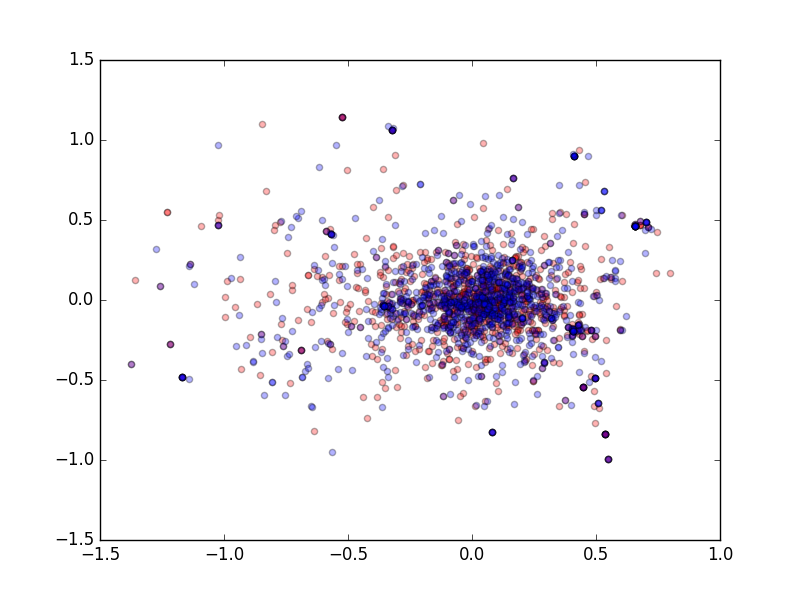
\includegraphics[width=0.5\linewidth]{../MovieFollowInformation/2Dmappingwithoutfollow.png}
  \caption{Movie picture}
  \label{fig:movie}
\end{figure}

We can see from figure \ref{fig:movie} that there is a high overlapping between red points and blue points which means they are not very different in 2 dimensions with 82.55\% information lost from the original data.

After running the algorithms 10 times, the average accuracy of the results is listed below:

Logistic Regression: 0.51

Decision Tree: 0.54

SVM: 0.53

Na\"{\i}ve Bayes: 0.53

KNN: 0.52

Boosting: 0.51

\section{Book Analysis}

We try our best to find some valuable results. Firstly, there are too many users from the sparse data set with no information on reading interests. In this case, we want to move the data with no reading interests. We adopted the method of SVD to find the user with more information on reading interests. Then we used some methods to analyze the user dataset after processing, such as K nearest neighbor and so on.

Our main idea on finding the reading interests in two group is that using map function in Java to traverse and read the files and use the lists to save the data. The algorithm is that traversing  the lists of two group. If there are books read by more than 2 persons, the data will be shown in the results. Otherwise, the data will be not shown in the result. The results of lists show the kinds of  books read by each group .If the lists show the data ,that is to say, the group is more likely reading the kinds of books. Then, we can compute the probability of the kinds of books read by each group. At the same time, we can do the same things between two group. Why do we set the value of 2?The main reason is that the data set is very sparse.

\begin{figure}[h]
  \centering
  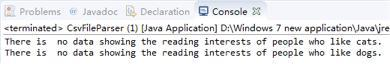
\includegraphics[width=0.7\linewidth]{../BookInformation/result.jpg}
  \caption{Book result}
  \label{fig:bookres}
\end{figure}

From discussed above, we find that there are no similar kinds of books read by the group of CatPeople or DogPeople. And there are also no similar kinds books read by both two groups. Our final result is that there are no special reading interests for two groups. The result of maven project in the Eclipse software is shown in the figure \ref{fig:bookres}.

\subsection{K-nearest neighbor}

\begin{figure}[h]
  \centering
  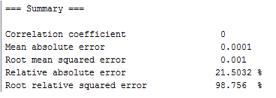
\includegraphics[width=0.7\linewidth]{../BookInformation/k-cat.jpg}
  \caption{The result of CatPeople using the  K-nearest neighbor}
  \label{fig:kcat}
\end{figure}

\begin{figure}[h]
  \centering
  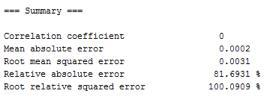
\includegraphics[width=0.7\linewidth]{../BookInformation/k-dog.jpg}
  \caption{The result of DogPeople using the  K-nearest neighbor}
  \label{fig:kdog}
\end{figure}

We use the other method to analyze the data set from two group. Also we want to  make our results more convinced. We use the software of  Weka, the method is K-nearest neighbor.  We want to get the better result by changing the value of K. However, the result of the methods did not change significantly. The result of CatPeople using K-nearest neighbor is shown in the figure \ref{fig:kcat}. At the same time, the result of DogPeople using K-nearest neighbor is shown in the figure \ref{fig:kdog}. We find that there are no special interests of reading in the two groups.


\section{Activity Analysis}

We use the same data processing technighes as before, and we also use the six algorithms to test this data and the average accuracy of the results is listed below:

Logistic Regression:  0.55

Decision Tree:  0.50

SVM:  0.53

Na\"{\i}ve Bayes:  0.50

KNN:  0.54

Boosting score:  0.55

To avoid the effect of culture or communities, we also try the algorithms on twitter users:

Logistic Regression:  0.54

Decision Tree:  0.53

SVM:  0.50

Na\"{\i}ve Bayes:  0.50

KNN:  0.50

Boosting score:  0.52

\section{Province Analysis}

We want to identify whether people living different province have a specific interest in cat or dogs, that is, whether the number of cat people and dog people is similar or not geographically.

We have the data where each category has about 100,000 items, and each item means one user and his/her specific living city.

Firstly we grouped those data using its city, but there are still too many cities, so we decided to group those data by provinces. We found a JSON file which lists all the province names with its secondary cities, and write a python file to automatically deal with those cities. It's not easy work because some cities have the same name and some cities use abbreviations.

So we get the data about the number of users which has cats or dogs for each province and use d3 to generate the data. We also count the number of cats minus the number of dogs for each province and tries to find the difference between the two categories.

\begin{figure}[h!]
  \centering
  \begin{subfigure}[b]{0.3\linewidth}
    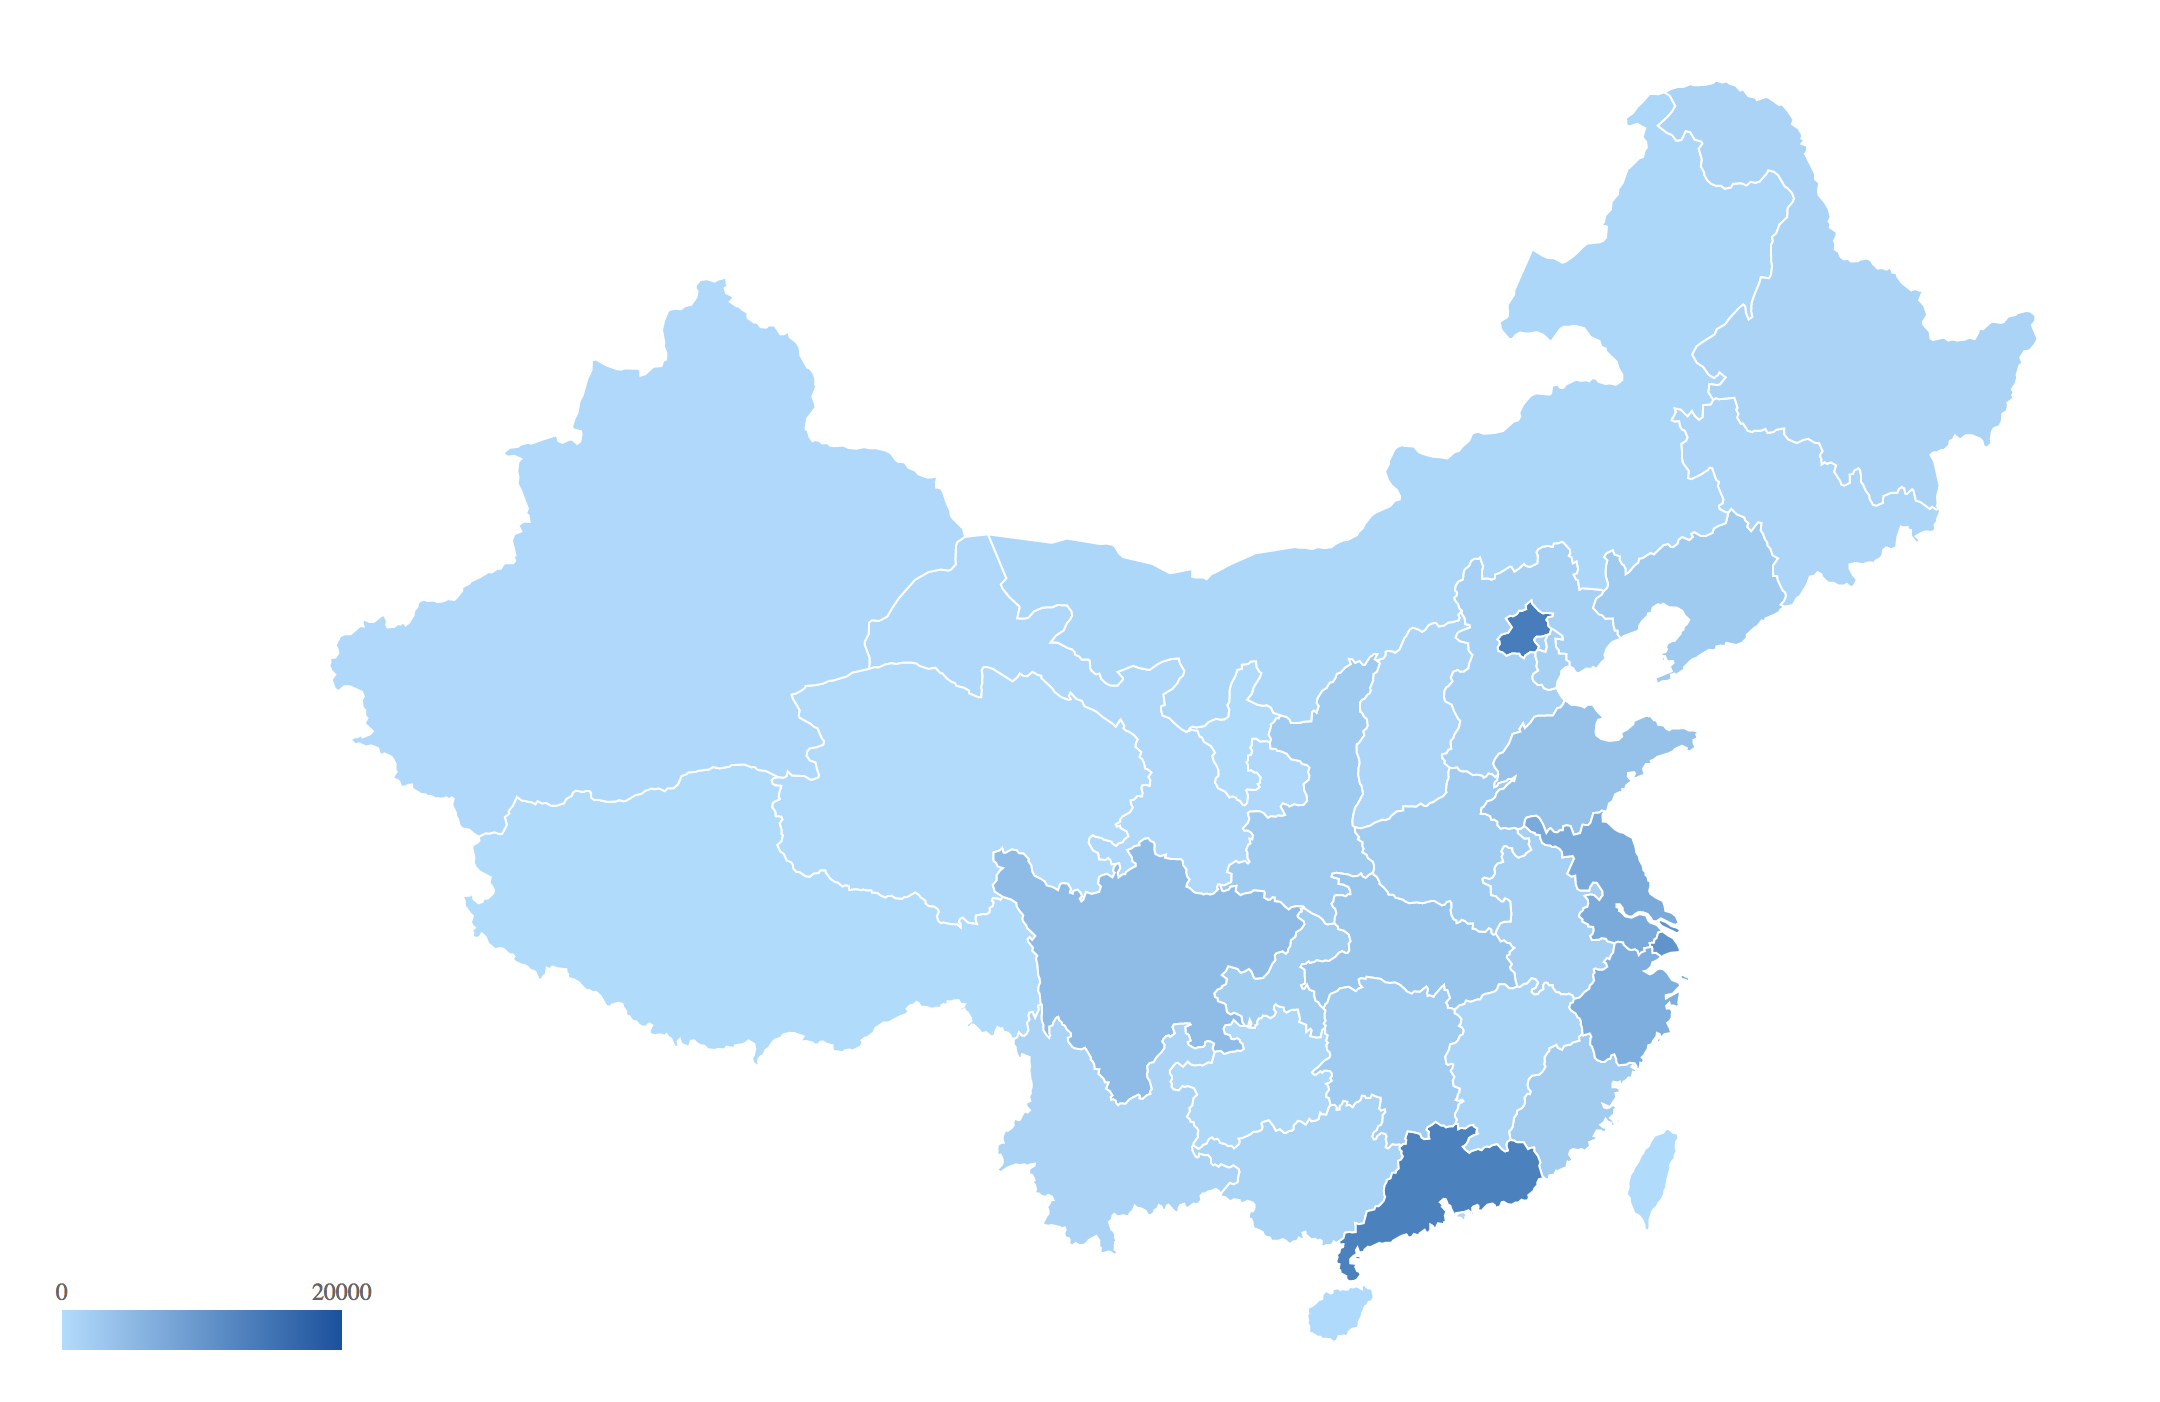
\includegraphics[width=\linewidth]{../Province/Cat_Province.png}
    \caption{The number of cat}
  \end{subfigure}
  \begin{subfigure}[b]{0.3\linewidth}
    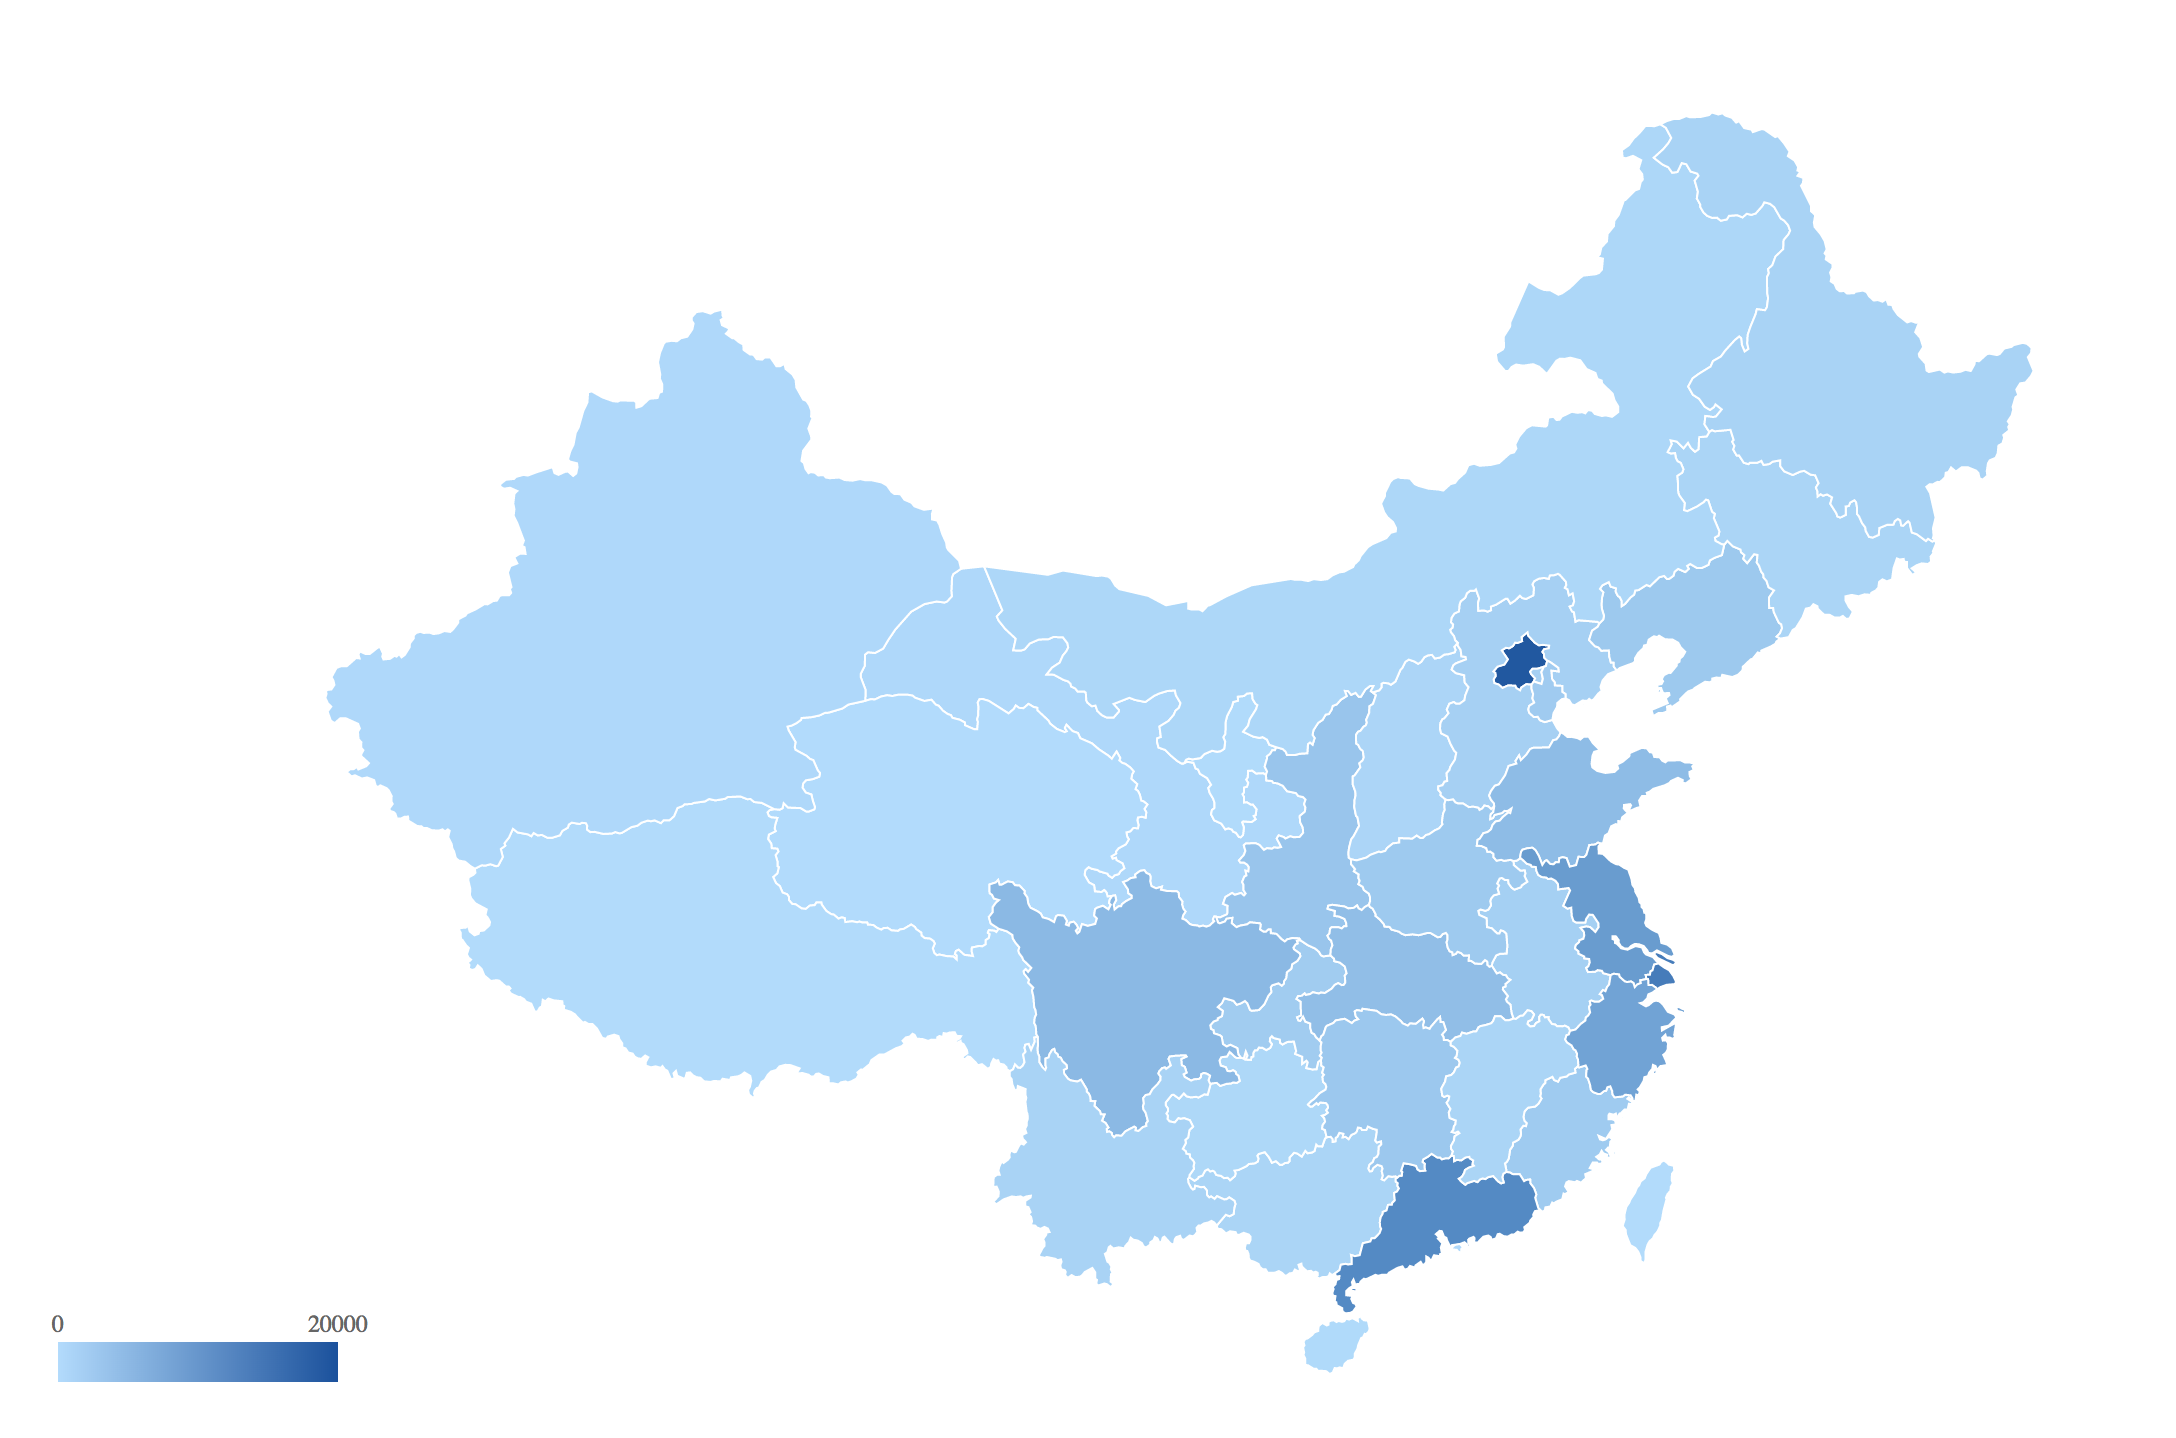
\includegraphics[width=\linewidth]{../Province/Dog_Province.png}
    \caption{The number of dog}
  \end{subfigure}
  \begin{subfigure}[b]{0.3\linewidth}
  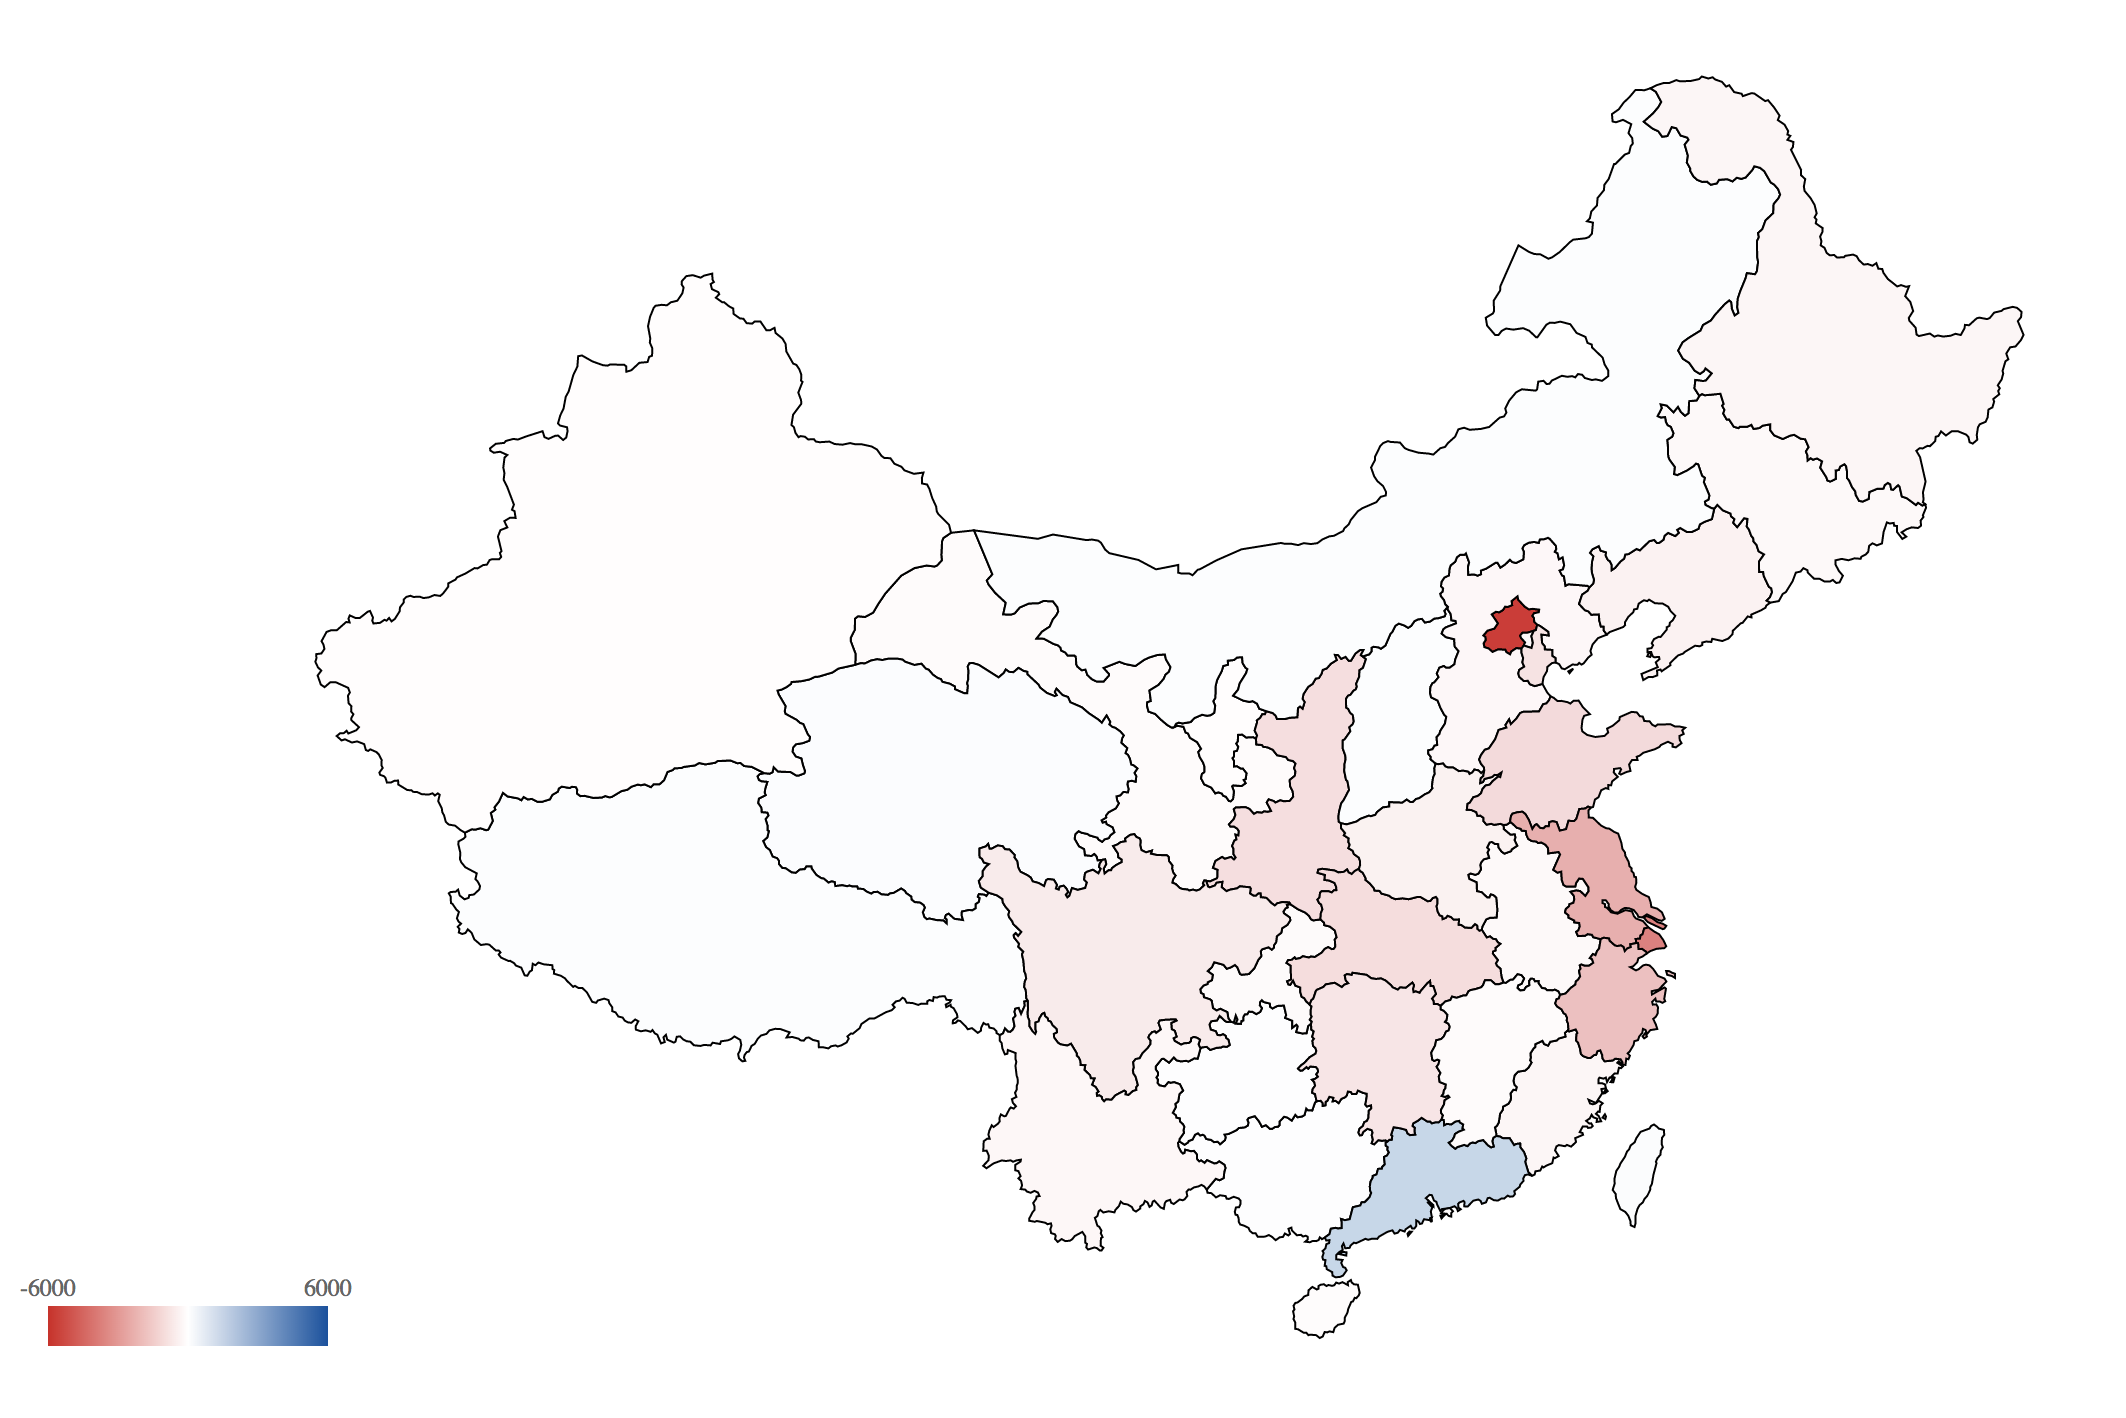
\includegraphics[width=\linewidth]{../Province/Diff_Province.png}
  \caption{The minus number}
  \end{subfigure}
  \caption{The province data}
  \label{fig:prov}
\end{figure}

The result is in figure \ref{fig:prov}, the first two pictures mean the number of cats and dogs in each province, and the last picture means the minus number (red means more dogs and blue means more cats).

It also seems that those provinces have more cats also have more dogs, which means that the two categories may have high correlations. So we use cat data as x axis and dog data as y axis and use linear regression, each node represent for a province.

\begin{figure}[h!]
  \centering
  \begin{subfigure}[b]{0.43\linewidth}
    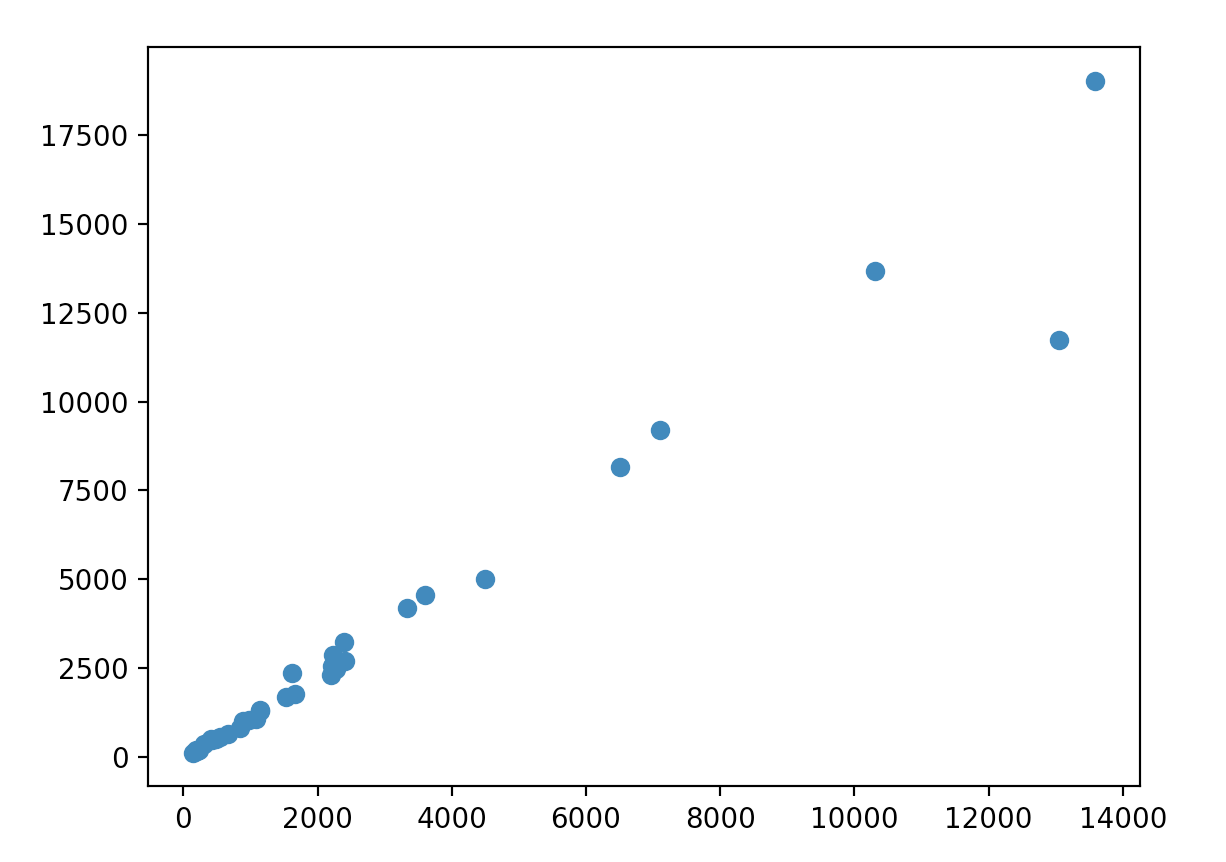
\includegraphics[width=\linewidth]{../Province/plot.png}
    \caption{Cat}
  \end{subfigure}
  \begin{subfigure}[b]{0.4\linewidth}
    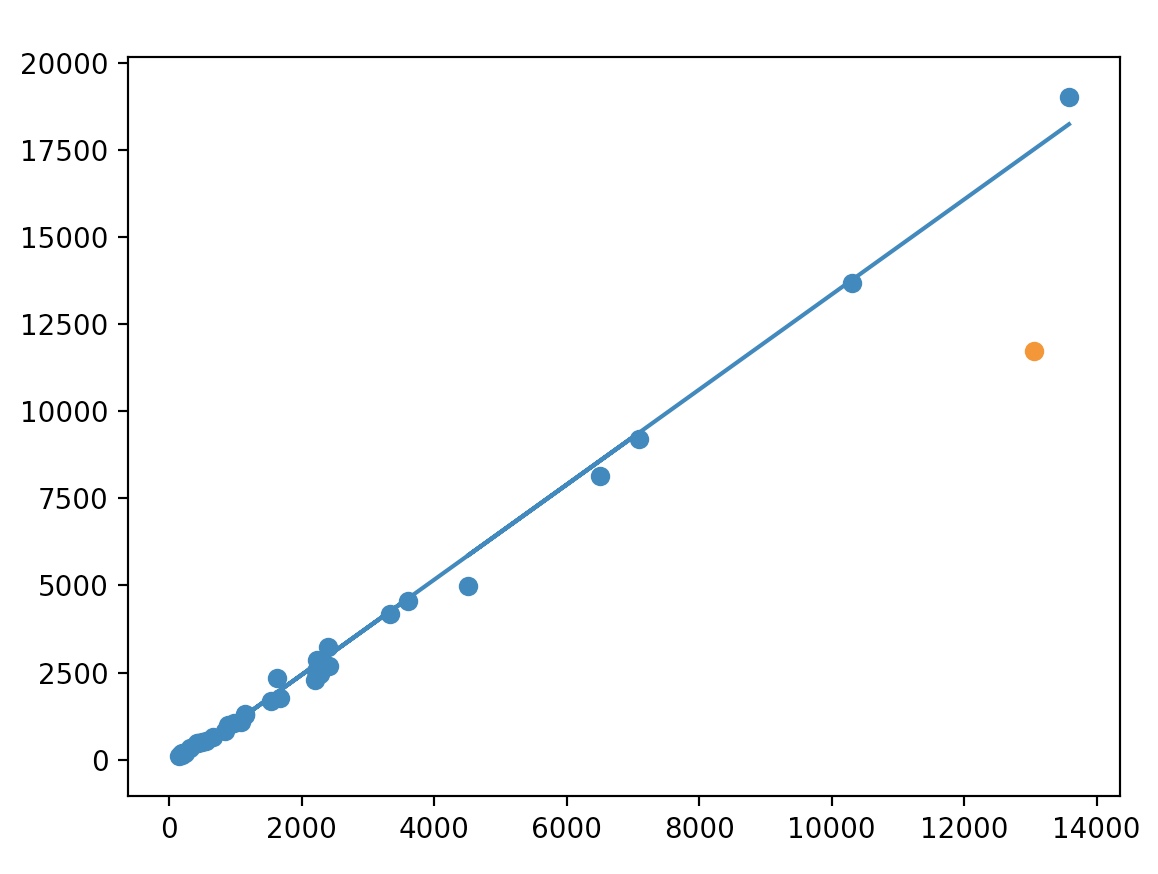
\includegraphics[width=\linewidth]{../Province/regression.png}
    \caption{Dog}
  \end{subfigure}
  \caption{Tag-cloud picture show their sentiment}
  \label{fig:regression}
\end{figure}

Figure \ref{fig:regression} can clearly show that Guangdong is an outlier, as guangdong has more cats than predicted.

In conclusion, almost all the province has little more dogs, but Guangdong is different from other cities and has more cats than predicted.

\section{Sentiment Analysis}
First, we crawl data From Twitter API. We search cat and dog hashtags as keywords instead of using cat and dog directly to avoid some meaningless tweets -- although it has cat or dog word but not directly related to cat or dogs.

We then do some data cleaning works, we removed those not-words refer to CNN sentence code.\footnote{Refer to: https://github.com/yoonkim/CNN\_sentence/blob/master/process\_data.py}, we also removed stopwords \footnote{Refer to: https://github.com/amueller/word\_cloud/blob/master/wordcloud/stopwords} and just keep real words\footnote{Refer to: https://www.nltk.org/book/ch02.html}.

As each tweet is too short, we combined tweets with same hashtags together and regard it as one document. Then there are two documents, one is about cats and the other one is about dogs. Because the two documents have many same words, using TF-IDF is a good choice for analysis which words are important for cats and dogs independently.

Then we decided to group those words into some groups. Sentiment analysis dictionary is a popular way to divide words, and words can be divided into two categories: negative and positive.

We choose the sentiment analysis dictionary\cite{hu2004mining}. The dictionary does not only have correct words, but also have many misspelled words, so it is more suitable to deal with social media content. What's more, the dictionary is highly correlated with the domain-specific orientations\cite{liu2010sentiment} and choosing a social media related dictionary is useful and necessary.

We count the weight of each category. After normalization, we generate the table below:

\begin{center}
\begin{tabular}{ |c|c|c| }
 \hline
  & cat & dog \\ \hline
 positive & 0.6 & 0.61 \\ \hline
 negative & 0.4 & 0.39 \\ \hline
\end{tabular}
\end{center}

We also use some visualization tools, such as tag-cloud to visualize those words.

\begin{figure}[h!]
  \centering
  \begin{subfigure}[b]{0.4\linewidth}
    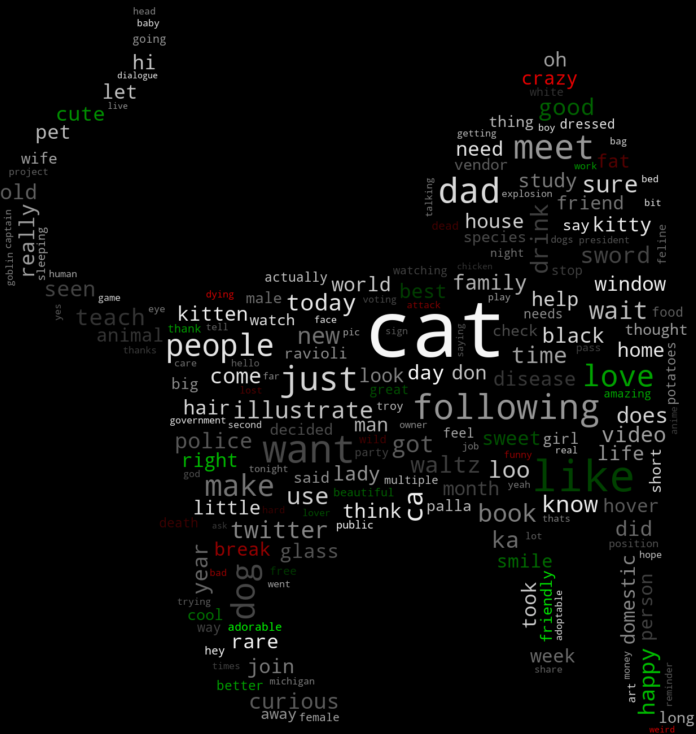
\includegraphics[width=\linewidth]{../Sentiment/tag_cat.png}
    \caption{Cat}
  \end{subfigure}
  \begin{subfigure}[b]{0.437\linewidth}
    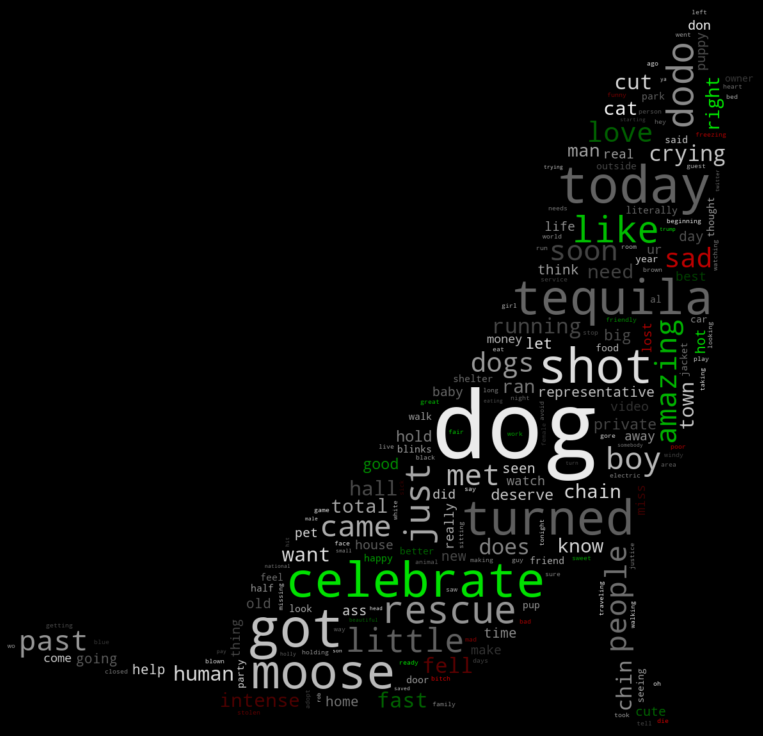
\includegraphics[width=\linewidth]{../Sentiment/tag_dog.png}
    \caption{Dog}
  \end{subfigure}
  \caption{Tag-cloud picture show their sentiment}
  \label{fig:tagcloud}
\end{figure}

Figure \ref{fig:tagcloud} shows the sentiment of each document, green means positive color and red means negative color. The majority of words are neutral, which means they are not negative or positive and be colored in grey.

\begin{figure}[h!]
  \centering
  \begin{subfigure}[b]{0.6\linewidth}
    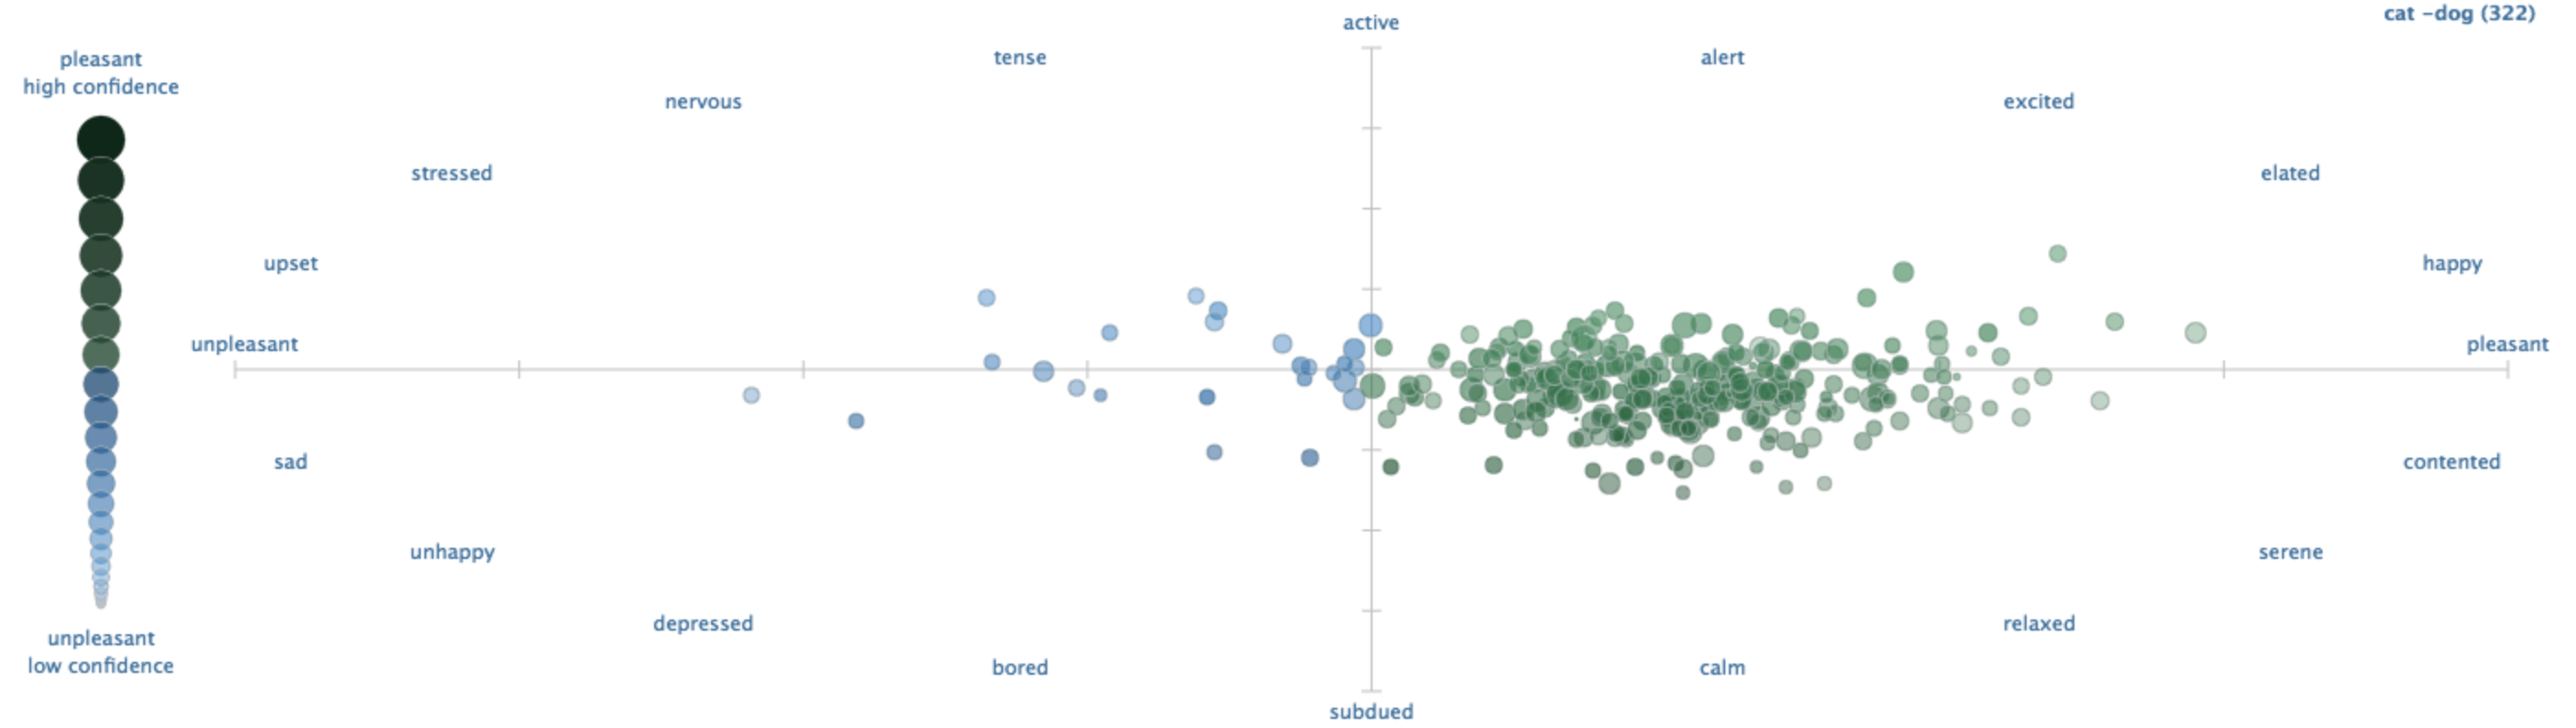
\includegraphics[width=\linewidth]{../Sentiment/cat.png}
    \caption{Cat}
  \end{subfigure}
  \begin{subfigure}[b]{0.6\linewidth}
    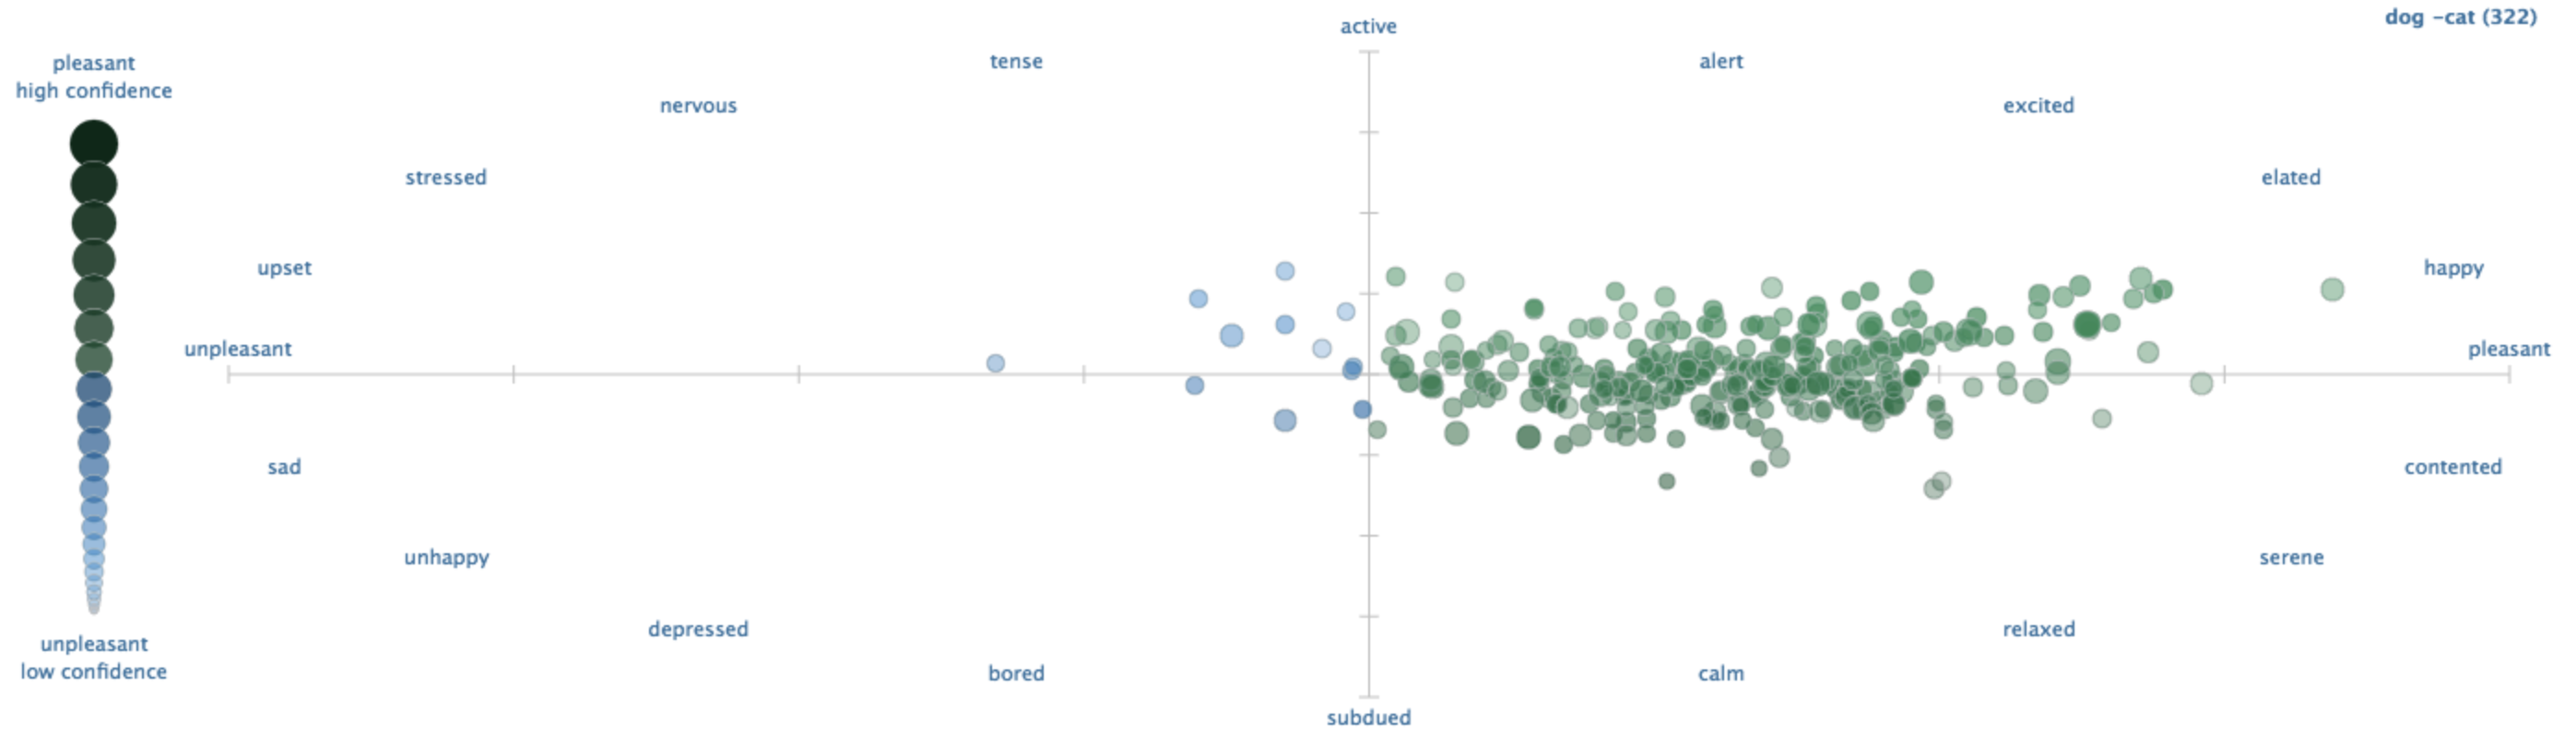
\includegraphics[width=\linewidth]{../Sentiment/dog.png}
    \caption{Dog}
  \end{subfigure}
  \caption{Another sentiment analysis result}
  \label{fig:twitter}
\end{figure}

There are also some other visualization tools to analysis words, This project \cite{healey} can analysis sentiment into two dimonsions, and result can be seen at figure \ref{fig:twitter}.

From the results above, we can see that although cat people seem a little more negative than dog people, they are both more positive than negative.


\section{Conclusion}
We can see that there is no model that can distinguish these two kinds of people in the respect of movie preference and degree activity. So, the truth is that cat people and dog people are just so same and not as different as what has been mentioned in the research of Facebook.

\section{Feedback}
\subsection{Meaning}
Q1. Why do you want to study this topic, and what is the purpose?

A: We first read a research from Facebook\cite{lada} which talks about the differences between cat people and dog people in some aspects such as the movie and book preference, marriage status and the number of friends based on the Facebook database which is not available to the public.

So we decided to try this idea on a famous social community 'Douban', where we can get users' information without any privacy issue, to see if we can prove the ideas in the research and not and try to find the specific differences between these two groups of people.

After realizing that 'Douban' data do not have clear differences, we decided to crawl data from Twitter to identify whether data from different platforms will influence the final result.

\subsection{Define}

Q2. If someone like both cat and dog, ow to define him/her? If someone joins both the cat and dog group, how to group this kind of users?

A: Because we want the difference between them to make user profile, we only extract people who like cat only and dog only and remove people who like them both.

Q3. How to classify cat and dog people? Do these people join the group really raising a dog/cat? How can you confirm that people join dog group as they like the dog more or their behavior represents they like a dog?

A: We choose the largest cat and dog groups in 'Douban' and define members in these groups as cat people and dog people because we consider that people who are willing to join a community to have a discussion with other people should share hobbies. People who love to talk about cats and dogs should be cat and dog people no matter having a real cat/dog or not. For example, people who love to talk about pop music doesn't mean they have to own pop music CDs. Besides, Douban is a place for people who share common hobbies to have discussions and comments. There is no reason that people who don't like dogs or cats but joining these groups and talk to other people. But if there are some people don't like cats or dogs but still join the groups, they are the noise information and we can ignore them because of the total number of members in each group is very large, up to 150, 000. We believe that the noise information should have only a small amount.

Q4. How to select the comparison criteria? I.e. books, movie, etc.

A: We get the idea from the Facebook research which indicates that cat people and dog people have different movie and book preference and number of friends. That is why we choose to get the users' movie and book preference and friends number as the feature of each user.

Q5. Do you try if there are more than two type people (cat and dog)?

A: There are billions of people in the world and each one is a unique one, so there should be countless types of people in the world actually. But for this topic, we only focus on the cat group and dog group.

\subsection{Analysis}
Q6. Which attributes are used in this analysis?

A: We collect top 100 movies and books he or she like the most for each user, put them together and do normalization to make the feature vector. In detail, we use the types of movies (37 kinds of movie types in total) and tags for books (over 3000 kinds of tags) to analyze their movie and book preference.

To analyze their activity from douban and Twitter both, we use three attributes: number of followers, number of followings, and number of groups he or she visits recently.

We also collect tweets with cat and dog hashtags from tweeter, and we regarded those tweets are about users showing their interest to those pets.

Q7. Is the data depends on the culture? (Facebook / Douban)

A: Actually not. We did additional analysis on the Twitter users and find that they have the same performance as users in Douban. Because the user profile is not available on Facebook, we cannot test our ideas on it.

Q8. Studies of people's gender, leisure time, marital status, and whether sharing a residence with others, etc. can efficiently improve the accuracy of the results. But these data involve personal privacy. If only considering the three aspects of this group, the results are not very convincing.

A: First of all, too many attributes may cause the curse of dimensionality. Choosing topic related attributes only can be helpful to the study. On the one hand, some information is private that we cannot get from the Internet even though they might be very helpful. On the other hand, what we want to study here is only the three aspects of these two groups because of the Facebook research we read, and we don't know what we will find exactly in the first place.

\subsection{Content}

Q9. Can the same algorithm be applied for analyzing with other feature except for sentiment, book and movie features? Can we categorize people into cat and dog by using their similar behavior?

A: There are many other useful attributes in the world that might be very helpful for the analysis but not available to the public. We have gained as many attributes as we can to make the model works. To distinguish two kinds of people, we need their different behavior instead of their similar behavior. The similar behavior only makes them looks the same and unable to find the difference.

\printbibliography

\end{document}
